\documentclass[11pt]{article}
\usepackage{coling2014}
\usepackage{times}
\usepackage{url}
\usepackage{latexsym}
\usepackage{graphicx}
\usepackage[utf8]{inputenc}
\bibliographystyle{acl}

%\setlength\titlebox{5cm}

% You can expand the titlebox if you need extra space
% to show all the authors. Please do not make the titlebox
% smaller than 5cm (the original size); we will check this
% in the camera-ready version and ask you to change it back.


\title{SentiMerge: Combining Sentiment Lexicons in a Bayesian Framework}

\author{Guy Emerson and Thierry Declerck \\
  DFKI GmbH \\
  Universität Campus \\
  66123 Saarbrücken \\
  {\tt \{guy.emerson, thierry.declerck\}@dfki.de} }

\date{}

\begin{document}
\maketitle

\begin{abstract}

Many approaches to sentiment analysis rely on a lexicon that labels words with a prior polarity. This is particularly true for languages other than English, where labelled training data is not easily available. Existing efforts to produce such lexicons exist, and to avoid duplicated effort, a principled way to combine multiple resources is required. In this paper, we introduce a Bayesian probabilistic model, which can simultaneously combine polarity scores from several data sources and estimate the quality of each source.  We apply this algorithm to a set of four German sentiment lexicons, to produce the SentiMerge lexicon, which we make publically available.  In a simple classification task, we show that this lexicon outperforms each of the underlying resources, as well as a majority vote model.

\end{abstract}

\blfootnote{
    \hspace{-0.65cm}  % space normally used by the marker
    This work is licensed under a Creative Commons 
    Attribution 4.0 International Licence.
    Page numbers and proceedings footer are added by
    the organisers.
    Licence details:
    \url{http://creativecommons.org/licenses/by/4.0/}
}

\section{Introduction}

\newcite{wiegand2011phd} describes sentiment analysis as the task of identifying and classifying opinionated content in natural language text.  There are a number of subtasks within this field, such as identifying the holder of the opinion, and the target of the opinion.

In this paper, however, we are concerned with the more specific task of identifying \emph{polar} language - that is, expressing either \emph{positive} or \emph{negative} opinions.  Throughout the rest of this paper, we will use the terms \emph{sentiment} and \emph{polarity} more or less interchangeably.

As \newcite{pang2008sentiment} explain, sentiment analysis has become a major area of research within natural language processing (NLP), with many established techniques, and a range of potential applications.  Indeed, in recent years there has been increasing interest in sentiment analysis for commercial purposes.

Despite the rapid growth of this area, there is a lack of gold-standard corpora which can be used to train supervised models, particularly for languages other than English.  Consequently, many algorithms rely on sentiment lexicons, which provide prior knowledge about which lexical items might indicate opinionated language.  Such lexicons can be used directly to define features in a classifier, or can be combined with a bootstrapping approach.

However, when presented with a number of overlapping and potentially contradictory sentiment lexicons, many machine learning techniques break down, and we therefore require a way to merge them into a single resource - or else a researcher must choose between resources, and we are left with a leaky pipeline between resource creation and application.  We review methods for combining sources of information in section~\ref{sec:rel}, and then describe four German sentiment lexicons in section~\ref{sec:data}.

To merge these resources, we first want to make them match as closely as possible, and then deal with the differences that remain.  We deal with the first step in section~\ref{sec:norm}, describing how to align the polarity scores in different lexicons so that they can be directly compared.  Then in section~\ref{sec:combine}, we describe how to combine these scores together.

We report results in section~\ref{sec:results}, including evaluation against a small annotated corpus, where our merged resource outperforms both the original resources and also a majority vote baseline.  Finally, we discuss distribution of our resource in section~\ref{sec:dist}, future work in section~\ref{sec:future}, and conclude in section~\ref{sec:conc}.


\section{Related Work} \label{sec:rel}

A general problem is how to deal with missing data - in our case, we cannot expect every word to appear in every lexicon.  \newcite{schafer2002missing} review techniques to deal with missing data, and recommend two approaches: maximum likelihood estimation and Bayesian multiple imputation. The latter is a Monte Carlo method, helpful when the marginal probability distribution cannot be calculated analytically. The probabilistic model presented in section~\ref{sec:model} is straightforward enough for marginal probabilities to be calculated directly, and we employ maximum likelihood estimation for this reason.

A second problem is how to combine multiple sources of information, which possibly conflict, and where some sources are more reliable than others.  This becomes particularly challenging in the case when no gold-standard data exists, and so the sources can not be evaluated directly.  \newcite{raykar2010crowds} discusses this problem from the point of view of crowdsourcing, where there are multiple expert views and no certain ground truth - but we can equally apply this in the context of sentiment analysis, viewing each source as an expert.  However, unlike their approach, our algorithm does not directly produce a classifier, but rather a newly labelled resource.

Confronted with a multiplicity of data sources, some researchers have opted to link resources together \cite{eckle2013cookbook}. Indeed, the lexicons we consider in section \ref{sec:data} have already been compiled into a common format by \newcite{declerck2014trendminer}. However, while linking resources makes it easier to access a larger amount of data, it does not solve the problem of how best to process it.

To the best of our knowledge, there has not been a previous attempt to use a probabilistic model to merge a number of sentiment lexicons into a single resource.


\section{Data Sources} \label{sec:data}

In the following subsections, we first describe four existing sentiment lexicons for German.  These four lexicons represent the data we have merged into a single resource, with a size comparison given in table~\ref{tab:size}, where we count the number of distinct lemmas, not considering parts of speech.  Finally, in section~\ref{sec:mlsa}, we describe the manually annotated MLSA corpus, which we use for evaluation.

\begin{table}[t]
\centering
    \begin{tabular}{|l|r|} \hline
	Lexicon        & \# Entries \\ \hline
	C\&K	& 8714 \\
	PolarityClues	& 9228 \\
	SentiWS	& 1896 \\
	SentiSpin	& 95572 \\ \hline
	SentiMerge	& 96918 \\ \hline
    \end{tabular}
\caption{Comparison of lexicon sizes}
\label{tab:size}
\end{table}


\subsection{Clematide and Klenner}

\newcite{clematide2010germanlex} manually curated a lexicon\footnote{\url{http://bics.sentimental.li/index.php/downloads}} of around 8000
words, based on the synsets in \emph{GermaNet}, a \emph{WordNet}-like database \cite{hamp1997germanet}. A semi-automatic approach was used to extend the lexicon, first
generating candidate polar words by searching in a corpus for coordination
with known polar words, and then presenting these words to human annotators.  We will refer to this resource as the C\&K lexicon.


\subsection{SentimentWortschatz} \label{sub:WortSchatz}

\newcite{remus2010sentiws} compiled a sentiment lexicon\footnote{\url{http://asv.informatik.uni-leipzig.de/download/sentiws.html}} from three data
sources: a German translation of \newcite{stone1966inquirer}'s \emph{General
Inquirer} lexicon, a set of rated product reviews, and a German collocation
dictionary. At this stage, words have binary polarity: positive or
negative. To assign polarity weights, they use a corpus to calculate
the mutual information of a target word with a small set of seed words.


\subsection{GermanSentiSpin} \label{sub:SentiSpin}

\newcite{takamura2005sentispin} produced SentiSpin, a sentiment lexicon
for English. It is so named becaused it applies the Ising Model of
electron spins. The lexicon is modelled as an undirected graph, with
each word type represented by a single node. A dictionary is used
to define edges: two nodes are connected if one word appears in the
other's definition. Each word is modelled as having either positive
or negative sentiment, analogous to electrons being spin up or spin
down. An energy function is defined across the whole graph, which
prefers words to have the same sentiment if they are linked together.
By using a small seed set of words which are manually assigned positive
or negative sentiment, this energy function allows us to propagate
sentiment across the entire graph, assigning each word a real-valued
sentiment score in the interval $\left[-1,1\right]$.

\newcite{waltinger2010reload} translated the SentiSpin resource into German\footnote{\url{http://www.ulliwaltinger.de/sentiment}}
using an online dictionary, taking at most three translations of each
English word.


\subsection{GermanPolarityClues}

\newcite{waltinger2010polclues} utilised automatic translations of two English
resources: the SentiSpin lexicon, described in section \ref{sub:SentiSpin}
above; and the Subjectivity Clues lexicon, a manually annotated lexicon
produced by \newcite{wilson2005subjclues}. The sentiment orientations
of the German translations were then manually assessed and corrected
where necessary, to produce a new resource.\footnote{\url{http://www.ulliwaltinger.de/sentiment}}


\subsection{MLSA} \label{sec:mlsa}

To evaluate a sentiment lexicon, separately from the general task of judging the sentiment of an entire sentence, we relied on the MLSA (Multi-Layered reference corpus for German Sentiment Analysis).  This corpus was produced by \newcite{clematide2012mlsa}, independently of the above four lexicons, and consists of 270 sentences annotated at three levels of granularity.  In the first layer, annotators judged the sentiment of whole sentences; in the second layer, the sentiment of words and phrases; and finally in the third layer, they produced a FrameNet-like analysis of each sentence.  The third layer also includes lemmas, parts of speech, and a syntactic parse.

We extracted the sentiment judgements of individual words from the second layer, using the majority judgement of the three annotators.  Each token was mapped to its lemmatised form and part of speech, using the information in the third layer.  In some cases, the lemma was listed as ambiguous or unknown, and in these cases, we manually added the correct lemma.  Additionally, we changed the annotation of nominalised verbs from nouns to verbs, to match the lexical entries.  Finally, we kept all content words (nouns, verbs, and adjectives) to form a set of test data.  In total, there were 1001 distinct lemma types, and 1424 tokens.  Of these, 378 tokens were annotated as having positive polarity, and 399 as negative.



\section{Normalising Scores\label{sec:norm}}

By considering positive polarity as a positive real number, and negative
polarity as a negative real number, all of the four data sources give
polarity scores between $-1$ and $1$. However, we cannot assume
that the values directly correspond to one another. For example, does
a $0.5$ in one source mean the same thing in another?  An example of the kind of data we are trying to combine is given in table~\ref{tab:lemma}, and we can see that the polarity strengths vary wildly between the sources.

\begin{table}[t]
\centering
    \begin{tabular}{|l|r|} \hline
	Lemma, POS        & vergöttern, \emph{V} \\ \hline
	C\&K	& 1.000 \\
	PolarityClues	& 0.333 \\
	SentiWS	& 0.004 \\
	SentiSpin	& 0.245 \\ \hline
    \end{tabular}
\caption{An example lemma, labelled with polarity strengths from each data source}
\label{tab:lemma}
\end{table}

The simplest model is to rescale scores linearly, i.e. for each
source, we multiply all of its scores by a constant factor. Intuitively,
the factors should be chosen to harmonise the values - a source with
large scores should have them made smaller, and a source with small
scores should have them made larger.


\subsection{Linear Rescaling for Two Sources}

To exemplify our method, we first restrict ourselves to the simpler
case of only dealing with two lexicons. Note that when trying to determine
the normalisation factors, we only consider words in the overlap between
the two; otherwise, we would introduce a bias according to what words
are considered in each source - it is only in the overlap that we
can compare them. However, once these factors have been determined,
we can use them to rescale the scores across the entire lexicon, including
items that only appear in one source.

We consider lemmas with their parts of speech, so that the same orthographic word with two possible parts of speech is treated as two independent lexical entries, in all of the following calculations.  However, we do not distinguish homophonous or polysemous lemmas within the same part of speech, since none of our data sources provided different sentiment scores for distinct senses.

For each word $i$, let $u_{i}$ and $v_{i}$ be the polarity scores
for the two sources. We would like to find positive real values $\lambda$
and $\mu$ to rescale these to $\lambda u_{i}$ and $\mu v_{i}$ respectively,
minimising the loss function $\sum_{i}\left(\lambda u_{i}-\mu v_{i}\right)^{2}$.
Intuitively, we are trying to rescale the sources so that the scores
are as similar as possible. The loss function is trivially minimised
when $\lambda=\mu=0$, since reducing the sizes of the scores also
reduces their difference. Hence, we can introduce the constraint that
$\lambda\mu=1$, so that we cannot simultaneously make the values
smaller in both sources. We would then like to minimise:

\[
\sum_{i}\left(\lambda u_{i}-\frac{1}{\lambda}v_{i}\right)^{2}
= \left|u\right|^{2}\lambda^{2}-2u.v+\left|v\right|^{2}\lambda^{-2}
\]

Note that we use vector notation, so that $\left|u\right|^{2}=\Sigma_{i}u_{i}^{2}$.
Differentiating this with respect to $\lambda$, we get:

\[2\lambda\left|u\right|^{2}-2\left|v\right|^{2}\lambda^{-3} = 0 \qquad \Rightarrow \qquad \lambda = \frac{\sqrt{\left|v\right|}}{\sqrt{\left|u\right|}} \]

However, observe that we are free to multiply both $\lambda$ and $\mu$ by a constant factor,
since this doesn't affect the relationship between the two sources, only the overall size of the polarity values.
By dividing by $\sqrt{\frac{\left|u\right|\left|v\right|}{n}}$, we derive
the simpler expressions $\lambda=\sqrt{n}\left|u\right|^{-1}$ and $\mu=\sqrt{n}\left|v\right|^{-1}$,
i.e. we should divide by the root mean square. In other words,
after normalising, the average squared polarity value is $1$ for
both sources.\footnote{In most sentiment lexicons, polarity strengths are at most 1.  This will no longer be true after this normalisation.}


\subsection{Rescaling for Multiple Sources}

For multiple sources, the above method needs tweaking.
Although we could use the overlap between all sources, this could
potentially be much smaller than the overlap between any two sources,
introducing data sparsity and making the method susceptible to noise.
In the given data, 10749 lexical items appear in at least two sources,
but only 1205 appear in all four. We would like to exploit this extra
information, but the missing data means that methods such as linear
regression cannot be applied.

A simple solution is to calculate the root mean square values for each pair of sources, and then average these values for each source.  These averaged values define normalisation factors, as a compromise between the various sources.


\subsection{Unspecified scores}

Some lexical items in the PolarityClues dataset were not assigned a numerical score, only a polarity direction.  In these cases, the task is not to normalise the score, but to assign one.  To do this, we can first normalise the scores of all other words, as described above.  Then, we can consider the words without scores, and calculate the root mean square polarity of these words in the other sources, and assign them this value, either positive or negative.



\section{Combining Scores} \label{sec:combine}

Now that we have normalised scores, we need to calculate a combined value. Here, we take a Bayesian approach, where we assume that there is a latent ``true'' polarity value, and each source is an observation of this value, plus some noise.


\subsection{Gaussian Model} \label{sec:model}

A simple model is to assume that we have a prior distribution of polarity values across the vocabulary, distributed normally. If we further assume that a language is on average neither positive nor negative, then this distribution has mean $0$. We denote the variance as $\sigma^{2}$. Each source independently introduces a linear error term, which we also model with a normal distribution: errors from source $a$ are distributed with mean $0$ and standard deviation $\sigma_{a}^{2}$, which varies according to the source.\footnote{Because of the independence assumptions, this model can alternatively be viewed as a Markov Network, where we have one node to represent the latent true polarity strengths, four nodes to represent observations from each source, and five nodes to represent the hyperparameters (variances)}


\subsection{Hyperparameter Selection} \label{sec:hyper}

If we observe a subset $S=\left\{ a_{1},\dots,a_{n}\right\} $ of
the sources, the marginal distribution of the observations will be
normally distributed, with mean $0$ and covariance matrix as shown
below. If the error variances $\sigma_{a}^{2}$ are small compared
to the background variance $\sigma^{2}$, then this implies a strong
correlation between the observations.

\[
\left(\begin{array}{cccc}
\sigma^{2}+\sigma_{a_{1}}^{2} & \sigma^{2} & \ldots & \sigma^{2}\\
\sigma^{2} & \sigma^{2}+\sigma_{a_{2}}^{2} & \cdots & \sigma^{2}\\
\vdots & \vdots & \ddots & \vdots\\
\sigma^{2} & \sigma^{2} & \cdots & \sigma^{2}+\sigma_{a_{n}}^{2}
\end{array}\right)
\]


To choose the values for $\sigma^{2}$ and $\sigma_{a}^{2}$, we can
aim to maximise the likelihood of the observations, i.e. maximise
the value of the above marginal distributions at the observed points.  This is in line with \newcite{schafer2002missing}'s recommendations. Such an optimisation problem can be dealt with using existing software, such as included in the SciPy\footnote{\url{http://www.scipy.org}} package for Python.


\subsection{Inference}

Given a model as above (whether or not the hyperparameters have been
optimised), we can calculate the posterior distribution of polarity
values, given the observations $x_{a_{i}}$. This again turns out
to be normally distributed, with mean $\hat{\mu}$ and variance $\hat{\sigma}^{2}$ given by:

\[
\hat{\mu} = \frac{\sum\sigma_{a_{i}}^{-2}x_{a_{i}}}{\sigma^{-2}+\sum\sigma_{a_{i}}^{-2}}
\]
\[
\hat{\sigma}^{-2} =  \sigma^{-2}+\sum\sigma_{a_{i}}^{-2}
\]

The mean is almost a weighted average of the observed polarity values, where each source has weight $\sigma_{a}^{-2}$. However, there is an additional term $\sigma^{-2}$ in the denominator - this means we can interpret this as a weighted average if we add an additional polarity value $0$, with weight $\sigma^{-2}$. This additional term corresponds to the prior.

The weights for each source intuitively mean that we trust sources more if they have less noise. The extra $0$ term from the prior means that we interpret the observations conservatively, skewing values towards $0$ when there are fewer observations. For example, if all sources give a large positive polarity value, we can be reasonably certain that the true value is also large and positive, but if we only have data from one source, then we are less certain if this is
true - our estimate $\hat{\mu}$ is correspondingly smaller, and the posterior variance $\hat{\sigma}^2$ correspondingly larger.



\section{Experiments and Results} \label{sec:results}


\subsection{Parameter Values} \label{sec:param}

The root mean square sentiment values for the sources were: C\&K 0.845; PolarityClues 0.608; SentiWS 0.267; and SentiSpin 0.560.  We can see that there is a large discrepancy between the sizes of the scores used, with SentiWS having the smallest of all.  It is precisely for this reason that we need to normalise the scores.

The optimal variances calculated during hyperparameter selection (section~\ref{sec:hyper}) were: prior 0.528; C\&K 0.328; PolarityClues 0.317; SentiWS 0.446; and SentiSpin 0.609. These values correlate with our intuition: C\&K and PolarityClues have been hand-crafted, and have smaller error variances; SentiWS was manually finalised, and has a larger error; while finally SentiSpin was automatically generated, and has the largest error of all, larger in fact than the variance in the prior. We would expect the polarity values from a hand-crafted source to be more accurate, and this appears to be justified by our analysis.


\subsection{Experimental Setup} \label{sec:eval}

The MLSA data (see section \ref{sec:mlsa}) consists of discrete polarity judgements - a word is positive, negative, or neutral, but nothing in between.\footnote{The annotation scheme also allows a further three labels: \emph{intensifier}, \emph{diminisher}, and \emph{shifter}. While this information is useful, we treat these values as neutral in our evaluation, since we are only concerned with words that have an inherent positive or negative polarity.} To allow direct evaluation against such a resource, we need to discretise the continuous range of polarity values; i.e. if the polarity value is above some positive threshold, we judge it to be positive; if it is below a negative threshold, negative; and if it is between the two thresholds, neutral.  To choose this threshold before evaluation, we calculated a Gaussian kernel density estimate of the polarity values in the entire lexicon, as shown in figure \ref{fig:density}.  There is a large density near 0, reflecting that the bulk of the vocabulary is not strongly polar; indeed, so that the density of polar items is clearly visible, we have chosen a scale that forces this bulk to go off the top of the chart.  The high density stops at around $\pm 0.23$, and we have accordingly set this as our threshold.

\begin{figure}[t]
\begin{centering}
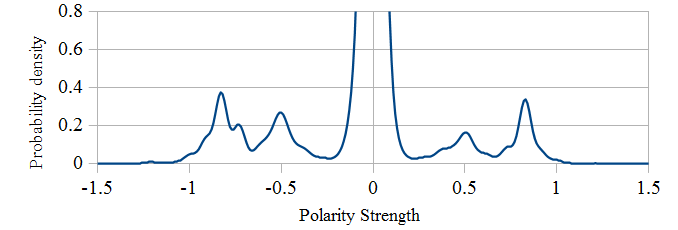
\includegraphics[scale=1]{density-wide.png}
\caption{Gaussian kernel density estimate}\label{fig:density}
\end{centering}
\end{figure}

We compared the merged resource to each of the original lexicons, as well as a "majority vote" baseline which represents an alternative method to combine lexicons.  This baseline involves considering the polarity judgements of each lexicon (\emph{positive}, \emph{negative}, or \emph{neutral}), and taking the most common answer.  To break ties, we took the first answer when consulting the lexicons in the following order, reflecting their reliability: C\&K, PolarityClues, SentiWS, SentiSpin.

For the automatically derived resources, we can introduce a threshold as we did for SentiMerge.  However, to make these baselines as competitive as possible, we optimised them on the test data, rather than choosing them in advance.  They were chosen to maximise the macro-averaged f-score.  For SentiWS, the threshold was 0, and for SentiSpin, 0.02.

Note that a perfect score would be impossible to achieve, since 31 lemmas were annotated with more than polarity type. These cases generally involve polysemous words which could be interpreted with different polarities depending on the context. Indeed, two words appeared with all three labels: \emph{Spannung} (tension) and \emph{Widerstand} (resistance).  In a political context, interpreting \emph{Widerstand} as positive or negative depends very much on whose side you support.  In such cases, a greater context is necessary to decide on polarity, and a lexicon simply cannot suffice.

\subsection{Evaluation on MLSA}

\begin{table}[t]
\centering
    \begin{tabular}{|l|ccc|} \hline
	Lexicon        & Precision & Recall       & F-score \\ \hline
	C\&K	& 0.754	& 0.733	& 0.743 \\
	PolarityClues	& 0.705	& 0.564	& 0.626 \\
	SentiWS	& \textbf{0.803}	& 0.513	& 0.621 \\
	SentiSpin	& 0.557	& 0.668	& 0.607 \\ \hline
	majority vote	& 0.548	& \textbf{0.898}	& 0.679 \\
	SentiMerge	& 0.708	& 0.815	& \textbf{0.757} \\ \hline
    \end{tabular}
\caption{Performance on MLSA, macro-averaged}
\label{tab:results}
\end{table}

We calculated precision, recall, and f-score (the harmonic mean of precision and recall) for both positive and negative polarity. We report the average of these two scores in \ref{tab:results}.  We can see that in terms of f-score, SentiMerge outperforms all four data sources, as well as the majority vote.  In applications where either precision or recall is deemed to be more important, it would be possible to adjust the threshold accordingly.  Indeed, by dropping the threshold to zero, we achieve recall of 0.894, competitive with the majority vote method; and by increasing the threshold to 0.4, we achieve precision of 0.755, competitive with the C\&K lexicon.  Furthermore, in this latter case, the f-score also increases to 0.760.  We do not report this figure in the table above because it would not be possible to predict such a judicious choice of threshold without peeking at the test data.  Nonetheless, this demonstrates that our method is robust to changes in parameter settings.

The majority vote method performs considerably worse than SentiMerge, at least in terms of f-score. Indeed, it actually performs worse than the C\&K lexicon, with noticeably lower precision. This finding is consistent with the results of \newcite{raykar2010crowds}, who argue against using majority voting, and who also find that it performs poorly.

The C\&K lexicon achieves almost the same level of performance as SentiMerge, so it is reasonable to ask if there is any point in building a merged lexicon at all. We believe there are two good reasons for doing this. Firstly, although the C\&K lexicon may be the most accurate, it is also small, especially compared to SentiSpin.  SentiMerge thus manages to exploit the complementary nature of the different lexicons, achieving the broad coverage of SentiSpin, but maintaining the precision of the C\&K lexicon for the most important lexical items.

Secondly, SentiMerge can provide much more accurate values for polarity strength than any human-annotated resource can. As \newcite{clematide2010germanlex} show, inter-annotator agreement for polarity strength is low, even when agreement for polarity direction is high.  Nonetheless, some notion of polarity strength can still be helpful in computational applications.  To demonstrate this, we calculated the precision, recall, and f-scores again, but weighting each answer as a function of the distance from the estimated polarity strength to the threshold.  With this weighted approach, we get a macro-averaged f-score of 0.852.  This is considerably higher than the results given in table~\ref{tab:results}, which demonstrates that the polarity scores in SentiMerge are useful as a measure of classification certainty.


\subsection{Manual Inspection}

In cases where all sources agree on whether a word is positive or negative, our algorithm simply serves to assign a more accurate polarity strength. So, it is more interesting to consider those cases where the sources disagree on polarity direction. Out of the 1205 lexemes for which we have data from all four sources, only 22 differ between SentiMerge and the C\&K lexicon, and only 16 differ between SentiMerge and PolarityClues.  One example is \emph{Beschwichtigung} (appeasement). Here we can see the problem with trying to assign a single numeric value to polarity - in a political context, \emph{Beschwichtugung} could be interpreted either as positive, since it implies an attempt to ease tension; or as negative, since it could be viewed as a sign of weakness.  Another example is \emph{unantastbar}, which again can be interpreted positively or negatively.

The controversial words generally denote abstract notions, or have established metaphorical senses. In the authors' view, their polarity is heavily context-dependent, and a one-dimensional score is not sufficient to model their contibution to sentiment.

In fact, most of these words have been assigned very small polarity values in the combined lexicon, which reflects the conflicting evidence present in the various sources. Of the 22 items which differ in C\&K, the one with the largest value in the combined lexicon is \emph{dominieren}, which has been assigned a fairly negative combined score, but was rated positive (0.5) in C\&K.


\section{Distribution} \label{sec:dist}

We are making SentiMerge freely available for download.  However, with the expanding number of language resources, it is becoming increasingly important to link resources together, as mentioned in section~\ref{sec:rel}.  For this reason, we are publishing our resource as part of the Linguistic Linked Open Data\footnote{\url{http://linguistics.okfn.org/resources/llod}} initiative.  In particular, we have decided to follow the specifications set forth by \newcite{buitelaar2013linked}, who propose a representation for sentiment resources based on Lemon \cite{mccraeJ2011lemon} and Marl \cite{westerski2011marl}.  Lemon\footnote{\url{http://lemon-model.net}} is a model for resource description which builds on LMF (Lexical Markup Framework),\footnote{\url{http://www.lexicalmarkupframework.org}} and facilitates combination of lexicons with ontologies.  Marl is an an ontology language designed for sentiment analysis, which has been fully implemented.\footnote{\url{http://www.gsi.dit.upm.es/ontologies/marl}}


\section{Future Work} \label{sec:future}

To align the disparate sources, a simple linear rescaling was used.  However, in principle any monotonic function could be considered.  A more general function that would still be tractable could be $u_i \mapsto \lambda u_i^\alpha$.

Furthermore, the probabilistic model described in section \ref{sec:model} makes several simplifying assumptions, which could be weakened or modified. For instance, we have assumed a normal distribution, with zero mean, both for the prior distribution and for the error terms. The data is not perfectly modelled by a normal distribution, since there are very clear bounds on the polarity scores, and some of the data takes discrete values.  Indeed, we can see in figure~\ref{fig:density} that the data is not normally distributed. An alternative choice of distribution might yield better results.

More generally, our method can be applied to any context where there are multiple resources to be merged, as long as there is some real-valued property to be aligned.


\section{Conclusion} \label{sec:conc}

We have described the merging of four sentiment lexicons into a single resource, which we have named SentiMerge.  To demonstrate the utility of the combined lexicon, we set up a word-level sentiment classification task using the MLSA corpus, in which SentiMerge outperformed all four of the underlying resources, as well as a majority vote baseline.  As a natural by-product of the merging process, we are also able to indirectly evaluate the quality of each resource, and the results match both intuition and the performance in the aformentioned classification task.  The approach we have taken requires no parameter setting on the part of the researcher, so we believe that the same method can be applied to other settings where different language resources present conflicting information.  This work helps to bridge the gap between resource creation efforts, which may overlap in scope, and NLP research, where researchers often want to use all available data.  Furthermore, by grounding our work in a well-defined Bayesian framework, we leave scope for future improvements using more sophisticated probabilistic models.  To allow the community at large to use and build on this work, we are making SentiMerge publically available for download, and are incorporating it into the Linguistic Linked Open Data initiative.


\section*{Acknowledgements}

This work was co-financed by the European Commission, within the FP7 ICT project TrendMiner,\footnote{\url{http://www.trendminer-project.eu}} under contract number 287863.  We would like to thank the authors of the all the resources mentioned in this paper for permission to use their data.  We also thank the anonymous reviewers for their helpful comments.


\bibliography{konvens2014}

\end{document}
